\subsection{Постановка задачи}
3.2. Построить кубический сплайн для функции, заданной в узлах интерполяции, предполагая, что сплайн имеет нулевую кривизну при $x=x_0$ и $x=x_4$. Вычислить значение функции в точке $x=X^*$.

{\bfseries Вариант:} 20
    \begin{equation}
		X^*=0.1
    \end{equation}
    \begin{center}
        \begin{tabular}{ |c|c|c|c|c|c| } 
			 \hline
			 $i$ & 0 & 1 & 2 & 3 & 4 \\ 
			 \hline
			 $x_i$ & -0.4 & -0.1 & 0.2 & 0.5 & 0.8 \\ 
			 \hline
			 $f_i$ & 1.5823 & 1.5710 & 1.5694 & 1.5472 & 1.4435 \\ 
			 \hline
        \end{tabular}
    \end{center}
\pagebreak

\subsection{Результаты работы}
\begin{figure}[h!]
\centering
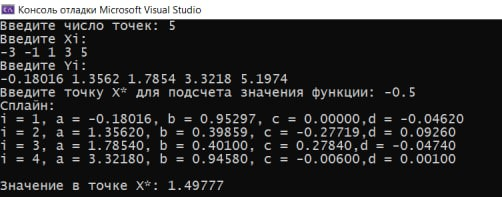
\includegraphics[width=.7\textwidth]{lab3.2}
\caption{Вывод в консоли}
\end{figure}


\subsection{Исходный код}
\lstinputlisting[title=\texttt{3-2.cpp}]{../stud/svoevolin/3-2.cpp}
\pagebreak